\documentclass[conference]{IEEEtran}
\IEEEoverridecommandlockouts
% The preceding line is only needed to identify funding in the first footnote. If that is unneeded, please comment it out.
\usepackage{cite}
\usepackage{amsmath,amssymb,amsfonts}
\usepackage{algorithmic}
\usepackage{graphicx}
\usepackage{textcomp}
\usepackage{xcolor}
\usepackage[hidelinks]{hyperref}
\usepackage{multirow}
\usepackage{float}
\usepackage[caption=false]{subfig}
\usepackage[font=small,labelfont=bf]{caption}
\usepackage[utf8]{inputenx}
\usepackage[croatian]{babel}
\def\BibTeX{{\rm B\kern-.05em{\sc i\kern-.025em b}\kern-.08em
		T\kern-.1667em\lower.7ex\hbox{E}\kern-.125emX}}
\begin{document}

\title{Bojenje crno-bijelih slika}


\author{\IEEEauthorblockN{1\textsuperscript{st} Luka Mucko}
		\IEEEauthorblockA{\textit{FER}}
		\and
		\IEEEauthorblockN{2\textsuperscript{nd} Filip Pankretić}
		\IEEEauthorblockA{\textit{FER}}
		\and
		\IEEEauthorblockN{3\textsuperscript{rd} Dominik Jambrović}
		\IEEEauthorblockA{\textit{FER}}
		\and
		\IEEEauthorblockN{4\textsuperscript{th} Velimir Kovačić}
		\IEEEauthorblockA{\textit{FER}}
		\and
		\IEEEauthorblockN{5\textsuperscript{th} Filip Perković}
		\IEEEauthorblockA{\textit{FER}}
		\and
		\IEEEauthorblockN{6\textsuperscript{th} Luka Glavinić}
		\IEEEauthorblockA{\textit{FER}}}
	

\maketitle

%\begin{abstract}
%Sažetak upisati ovdje
%\end{abstract}

%\begin{IEEEkeywords}
%kljucne, rijeci, upisati, ovdje
%\end{IEEEkeywords}

\section{Uvod}
% 1. Uvod/Motivacija
Bojenje crno-bijelih slika zadatak je u području računalnog vida, a glavna mu je primjena restauracija povijesnih fotografija kako bi njihov prikaz bio što vjerniji stvarnosti. Tradicionalne metode bojenja slika iziskuju značajnu količinu ručnog rada, stručnosti i vremena. S razvojem dubokog učenja i konvolucijskih neuronskih mreža, postalo je moguće automatizirano bojenje slika, što smanjuje potrebu za ručnim radom i omogućuje bržu i učinkovitiju obradu slika. U ovom radu bit će opisano korištenje generativnih modela, posebno generativnih suparničkih mreži (engl. \textit{Generative Adversarial Networks} - GAN), za bojanje crno-bijelih slika. Ta metoda uključuje dva modela: generator, koji stvara obojene slike iz nasumičnog vektora, i diskriminator, koji pokušava razlikovati generirane slike od stvarnih. Specifično je opisano korištenje uvjetnog GAN-a (engl. \textit{conditional} GAN - cGAN), koji na ulazu diskriminatora i generatora dodaje crno-bijelu reprezentaciju slike kao uvjetni vektor. Ovakav pristup omogućuje generiranje visoko kvalitetnih obojenih slika koje su u većini slučajeva vrlo slične onim stvarnima.

\section{Pregled postojećih pristupa}
% 2. Pregled postojećih pristupa
Razne su tehnike i metode bojenja crno-bijelih slika nastajale tijekom godina. Tradicionalne metode bojenja oslanjale su se na ručni unos i različite algoritme za propagaciju boje. Jedan je primjer \textit{Scribble-Based Colorization}\cite{li2018overview}, gdje korisnik dodaje boje na određene dijelove slike, a algoritam zatim te boje širi po slici.

S razvojem dubokog učenja, došlo je do značajnog napretka u automatizaciji procesa bojenja. Rana istraživanja koristila su konvolucijske neuronske mreže (CNN), pri čemu je mreža učila mapirati crno-bijele slike u obojene slike na temelju velikog skupa obojenih slika. Jedan primjer te metode predstavlja istraživanje \textit{Colorful Image Colorization}\cite{zhang2016colorful} iz 2016., u kojem su autori koristili konvolucijsku neuronsku mrežu za predikciju distribucije boja za svaki piksel crno-bijele slike. Pojavom GAN-ova i cGAN-ova kvaliteta generiranih obojenih slika ponovno je znatno poboljšana. Rad \textit{Image-to-Image Translation with Conditional Adversarial Networks}\cite{isola2018imagetoimage} iz 2017. ilustrira korištenje cGAN-a za različite zadatke translacije sa slike na sliku, uključujući i bojanje crno-bijelih slika.

Nedavno uvedene nadogradnje uključuju korištenje \textit{U-Net} arhitekture neuronske mreže u generatoru, koja omogućuje bolje dohvaćanje konteksta i detalja u slici dodavanjem preskočnih veza (engl. \textit{skip connections}) između slojeva kodera i dekodera. To dovodi do kvalitetnijih rezultata, posebno u zadacima gdje je očuvanje strukturalnih detalja ključno.

Ovaj projekt koristi cGAN arhitekturu s U-Net generatorom i konvolucijskom mrežom kao diskriminatorom kako bi postigao visoku kvalitetu obojenih slika. Ovaj pristup omogućuje iskorištavanje prednosti suvremenih tehnika dubokog učenja za postizanje vrhunskih rezultata u bojanju crno-bijelih slika.


\section{Opis skupa podataka}
% 3. Skup podataka

U ovome radu koristili smo skup podataka COCO 2017.
COCO (Common Objects in Context) 2017 skup je podataka koji je široko korišten u području računalnog vida. Dizajniran je s ciljem omogućavanja unapređenja razvoja algoritama za prepoznavanje objekata, segmentaciju, detekciju i opisivanje slika.

COCO 2017 sadrži više od 200 000 primjera. U našem radu, za učenje smo koristili 118 287 primjera, dok je za testiranje korišteno 40 670 primjera.
Slike iz skupa podataka prikupljene su iz različitih scenarija svakodnevnog života - cilj je prikazivanje objekata u njihovoj prirodnoj okolini tj. kontekstu.
Skup podataka sadrži oznake za 80 različitih razreda objekata, uključujući ljude, životinje, vozila, kućanske predmete i brojne druge.

\begin{figure}[H]
    \centering
    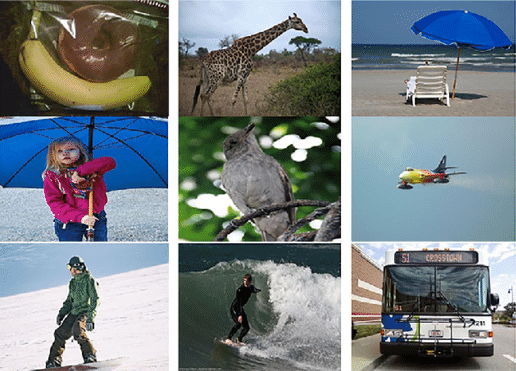
\includegraphics[width=0.9\linewidth]{imgs/coco_primjeri.png}
    \caption{Primjer slika iz skupa COCO 2017. Preuzeto iz\cite{bourouis2021color}.}
    \label{fig:slike_COCO}
\end{figure}

COCO 2017 ne koristi se samo za klasifikaciju pa stoga sadrži i neke pomoćne oznake.
Među njima su oznake granica objekata tj. okviri (engl. \textit{bounding boxes}), kao i
precizne maske segmentacije za svaki objekt - ovo omogućava učenje modela za segmentaciju.
Dodatno, skup podataka sadrži i oznake ključnih točaka za ljudsko tijelo, uključujući oznake ramena, laktova te koljena.
Svaka slika ima više tekstualnih opisa, što je korisno za zadatak opisivanja slika, kao i učenje jezičnih modela vezanih uz slike.

\section{Arhitektura cGAN}
% 4. GAN -> cGAN

Generativne suparničke mreže\cite{goodfellow2020generative} razvio je istraživački tim pod vodstvom Iana Goodfellowa 2014. godine. Ova arhitektura sastoji se od dvije mreže koje rade jedna protiv druge (suparnički). Mreža generator na temelju nasumičnog vektora (najčešće uzorkovanog iz normalne razdiobe) treba generirati sliku koja bi idealno odgovarala distribuciji stvarnih podataka. S druge strane, diskriminator za slike na ulazu treba identificirati radi li se o stvarnoj ili umjetnoj (generiranoj) slici. 

\begin{figure}[H]
    \centering
    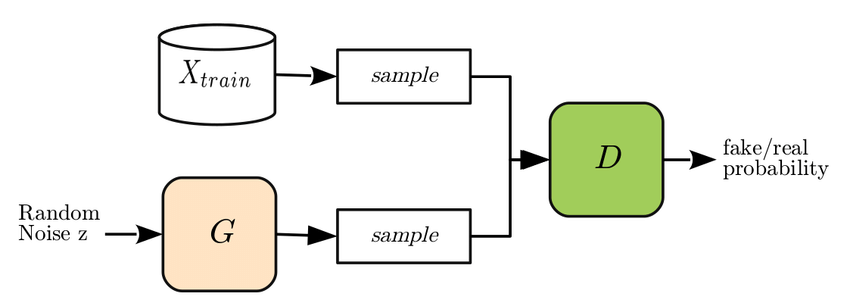
\includegraphics[width=0.9\linewidth]{imgs/gan.png}
    \caption{Arhitektura GAN. Preuzeto iz\cite{hayes2017logan}.}
    \label{fig:arhitektura_gan}
\end{figure}

Tijekom učenja, diskriminator želi maksimizirati svoju pouzdanost klasifikacije - idealno, diskriminator bi za stvarne slike na izlazu dao vrijednost 1, dok bi za umjetne slike dao vrijednost 0. Istovremeno, generator želi generirati slike za koje će diskriminator što pouzdanije reći da su stvarne. Vidimo da je ovo igra s nultim zbrojem (engl. \textit{zero-sum game}).

Za generator smo koristili arhitekturu zvanu U-Net\cite{ronneberger2015unet}.
U-Net je konvolucijska neuronska mreža koja je prvobitno razvijena za zadatke segmentacije medicinskih slika, ali se s vremenom pokazala vrlo učinkovitom i u različitim drugim zadacima računalnog vida, uključujući segmentaciju, translaciju sa slike na sliku i bojanje slika.
Arhitektura se sastoji od dva glavna dijela: kodera (downsampling path) i dekodera (upsampling path), koje zajedno formiraju oblik slova "U". Koder i dekoder oblikovali smo kao zasebne blokove u našem konačnom modelu.

Dodatno, arhitektura U-Net uključuje preskočne veze (engl. \textit{skip connections}) između odgovarajućih slojeva kodera i dekodera. One omogućuju prijenos niskorazinskih značajki, čime se poboljšava točnost i preciznost rekonstrukcije slike.
Preskočne veze ostvaruju se konkateniranjem značajki iz odgovarajućeg sloja kodera sa značajkama iz odgovarajućeg sloja dekodera.

\begin{figure}[H]
    \centering
    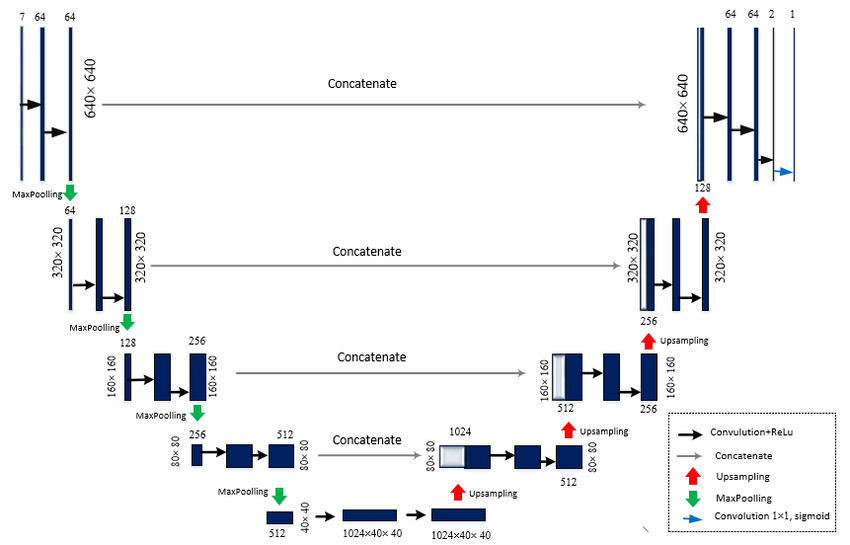
\includegraphics[width=0.9\linewidth]{imgs/unet.png}
    \caption{Arhitektura U-Net. Preuzeto iz\cite{raudonis2021fast}.}
    \label{fig:arhitektura_unet}
\end{figure}

Koder se sastoji od niza konvolucijskih blokova. Svaki od tih blokova sadrži dva konvolucijska sloja s aktivacijom ReLU, kao i sloj sažimanja maksimumom (engl. \textit{max-pooling}) za smanjenje dimenzija i povećanje receptivnog polja.
Svaki blok smanjuje prostorne dimenzije i povećava broj kanala, što omogućuje modelu da uči sve složenije značajke.

Dekoder se također sastoji od niza konvolucijskih blokova. Ipak, kako bi postigli povećanje prostornih dimenzija, u dekoderskim blokovima koristi se transponirana konvolucija. Dodatno, koriste se i slojevi normalizacije po grupi (engl. \textit{batch normalization}). Kao aktivacijska funkcija, u dekoderu se koristi propusna zglobnica (engl. \textit{Leaky ReLU}). Osim transponirane konvolucije, za povećanje prostornih dimenzija se može koristiti i interpolacija - npr. bilinearna interpolacija. Svaki blok povećava prostorne dimenzije i smanjuje broj kanala, obnavljajući detalje slike.

Uvjetne generativne suparničke mreže (engl. \textit{Conditional Generative Adversarial Networks} - cGAN) napredna su varijanta GAN-ova koja uvodi dodatne informacije u proces generiranja, ali i klasificiranja podataka. Ove mreže omogućuju generiranje uzoraka uvjetovanih određenim unosom, kao što su slike, oznake razreda, tekstualni opisi ili druge vrste podataka. cGAN-ovi su vrlo korisni za zadatke gdje postoji potreba za kontroliranim generiranjem primjeraka poput bojanja slika, translacije sa slike na sliku i generiranja slika prema tekstualnim opisima. U našem radu, kao uvjetni vektor na ulaz generatora dovodimo crno-bijelu (engl. \textit{grayscale}) sliku.

\section{Mjere dobrote}
% 5. Opis metrika

Kada govorimo o evaluaciji performansi generativnih modela, postoje dva pristupa.
Prvi od pristupa je vizualna procjena kvalitete - generirane slike ocjenjuju ljudi.
Pošto je ovaj pristup veoma subjektivan, uvedene su brojne mjere dobrote tj. kvantitativne metrike.
Ako je u pitanju zadatak poput bojanja slika gdje imamo očekivani izlaz, mogu se koristiti mjere poput srednje kvadratne pogreške (engl. \textit{Mean Squared Error - MSE}) i mjere indeksa strukturalne sličnosti (engl. \textit{Structural Similarity Index Measure} - SSIM). 
U našem radu koristili smo mjere IS (engl. \textit{Inception Score}) i FID (engl. \texit{Fréchet Inception Distance}).

IS\cite{salimans2016improved} je mjera dobrote koja se koristi za procjenu kvalitete slika generiranih generativnim modelima, posebno GAN-ovima. Mjera koristi prednaučenu mrežu Inception v3\cite{szegedy2015going} za izračunavanje rezultata, a fokus mjere su dva ključna aspekta generiranih slika: kvaliteta i raznolikost.
Konkretno, kvaliteta generiranih slika manifestira se visokom pouzdanošću klasifikacije mreže Inception v3 za pojedine slike. Drugim riječima, za svaku generiranu sliku, model bi na izlazu trebao dati distribuciju vjerojatnosti koja je fokusirana na jedan razred. Oba aspekta možemo kvantificirati koristeći KL-divergenciju izračunatu između distribucija vjerojatnosti za pojedine slike te distribucije marginaliziranih vjerojatnosti za sve razrede.

\begin{figure}[H]
    \centering
    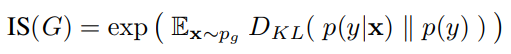
\includegraphics[width=0.9\linewidth]{imgs/IS_formula.png}
    \caption{Formula za izračun IS-a.}
    \label{fig:is_formula}
\end{figure}

FID\cite{heusel2017gans} je mjera dobrote koja se također koristi za procjenu kvalitete generiranih slika. Kroz godine, ova mjera postala je standard u evaluaciji generativnih modela, posebno GAN-ova. FID mjeri sličnost između distribucija stvarnih i generiranih slika. Konkretno, za izračun mjere FID koristi se Fréchetova udaljenost između dvije multivarijatne normalne distribucije. Pritom distribucije modeliraju značajke iz posljednjeg sloja mreže Inception v3 - jedna distribucija modelira značajke za stvarne slike, dok druga distribucija modelira značajke za generirane slike.

\begin{figure}[H]
    \centering
    
\includegraphics[width=0.9\linewidth]{imgs/FID_formula.png}
    \caption{Formula za izračun FID-a.}
    \label{fig:fid_formula}
\end{figure}

\section{Eksperimentalni rezultati}
% 6. Experimentalni rezultati i metrike

Slike za učenje modela na početku smo pretvorili u CIELAB prostor boja. Generator za zadanu crno-bijelu sliku (L komponentu originalne obojene slike) treba generirati komponente A i B.
Na temelju generiranih A i B komponenti, stvara se obojena slika u CIELAB prostoru boja koja se prosljeđuje diskriminatoru.

Model smo učili 200 epoha. Za gubitak diskriminatora koristili gubitak unakrsne entropije, a za gubitak generatora koristili smo gubitak diskriminatora, kao i rekonstrukcijski gubitak (L1 udaljenost između umjetne i stvarne slike). Kao optimizator smo za obje mreže koristili optimizator Adam s početnom stopom učenja $2 \cdot 10^{-4}$ .
Nakon učenja modela, generator smo koristili za bojenje crno-bijelih slika. 

Usporedno su prikazane: crno-bijela slika,  slika obojena modelom cGAN i konačno stvarna slika u boji. Na slici \ref{fig:slike_skup} prikazan je izbor od nasumičnih 8 slika iz skupa COCO 2017 koje je model vidio pri učenju. Osim ovoga, prikazan je i izbor od 8 nasumičnih slika iz privatnih galerija ili s interneta koje model nije vidio pri učenju, na slici \ref{fig:slike_vlastite}.

\begin{figure}[H]
    \centering
    \includegraphics[width=0.9\linewidth]{imgs/slike_skup.png}
    \caption{Primjer obojenih slika iz skupa COCO 2017}
    \label{fig:slike_skup}
\end{figure}


\begin{figure}[H]
    \centering
    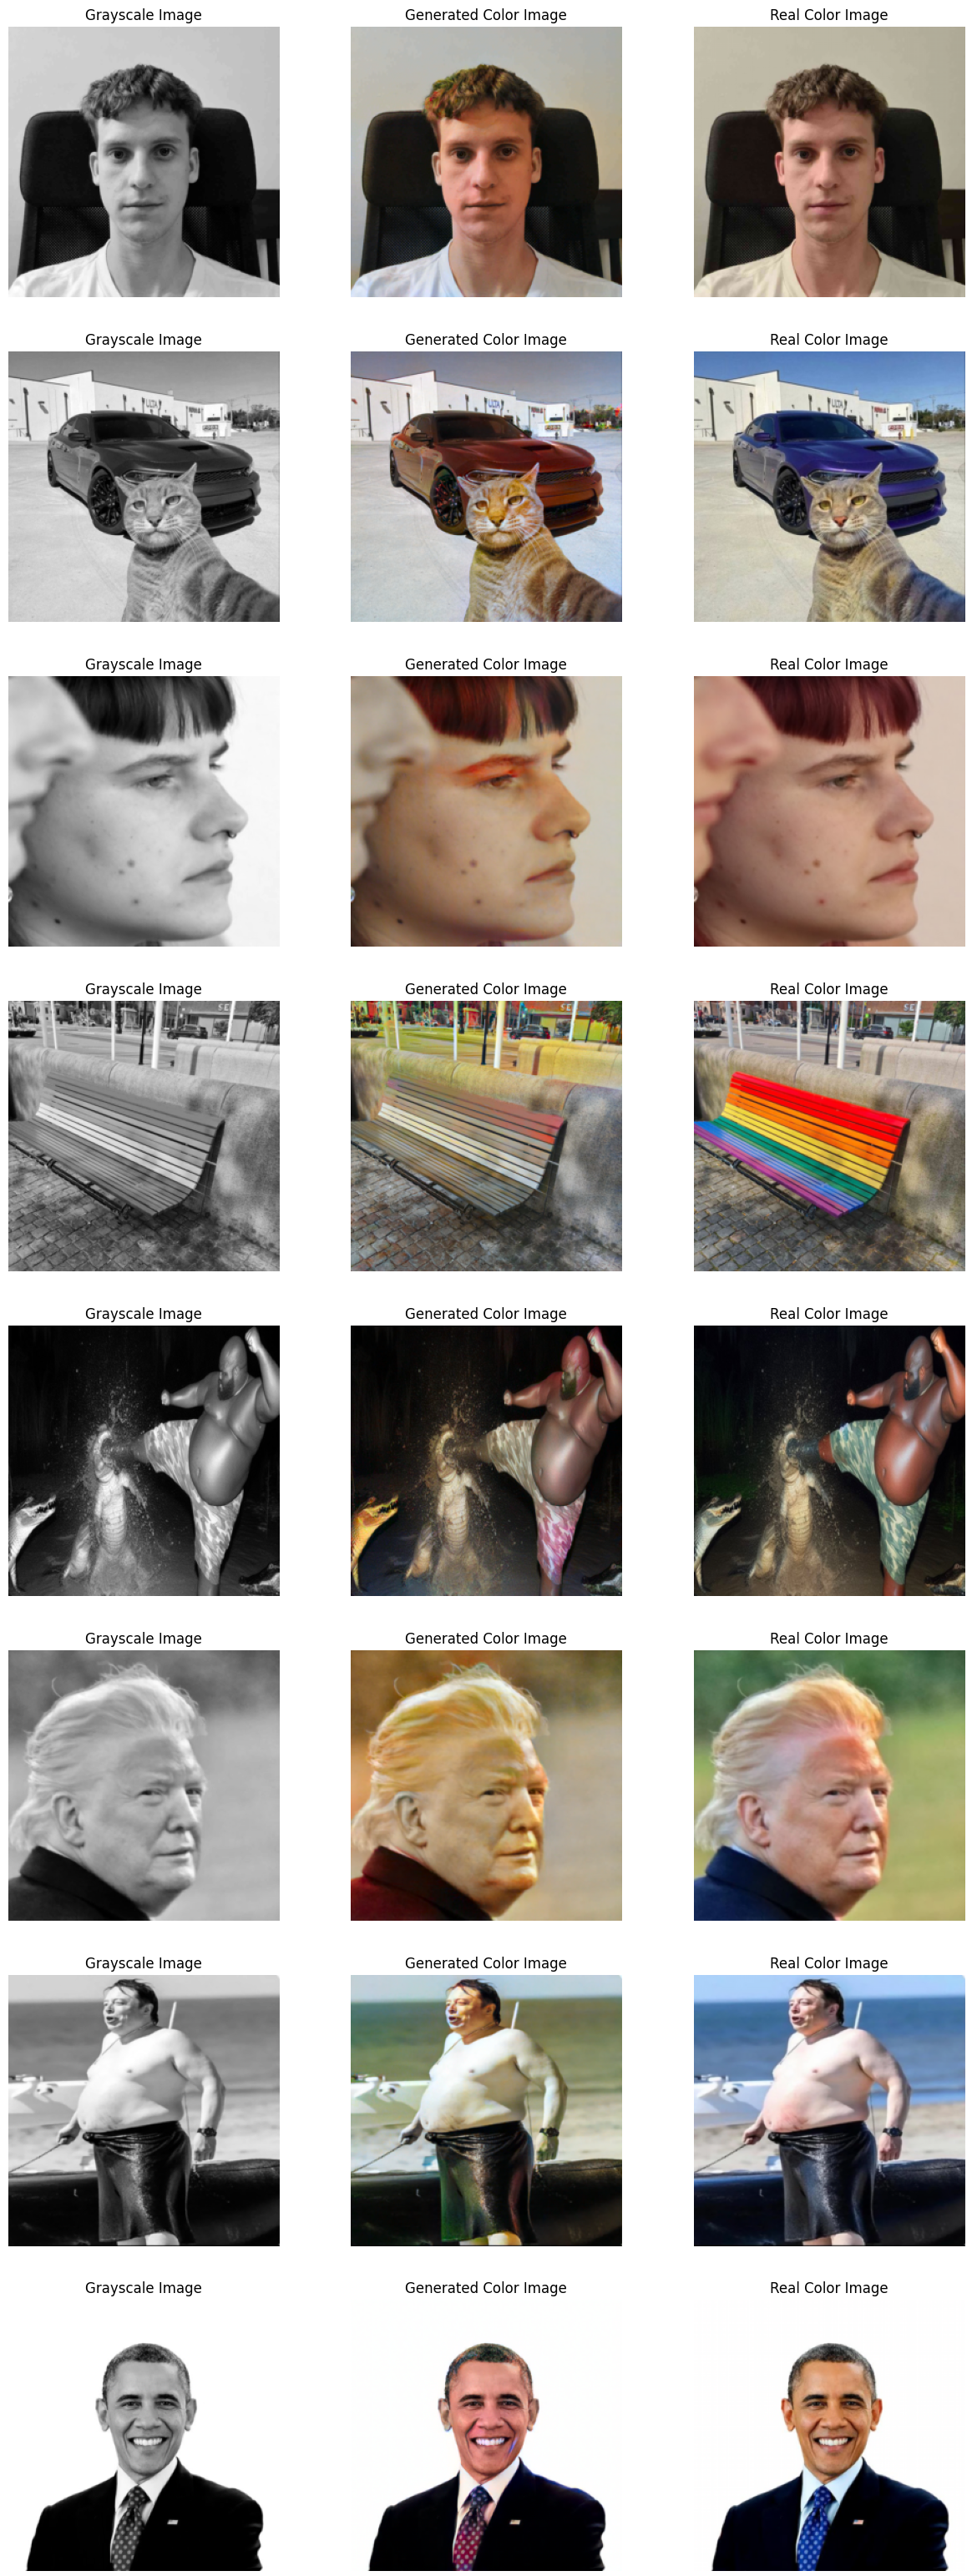
\includegraphics[width=0.9\linewidth]{imgs/slike_vlastite.png}
    \caption{Primjer obojenih vlastitih slika}
    \label{fig:slike_vlastite}
\end{figure}

Na temelju ovog uskog izbora slika, može se primijetiti da model mnogo bolje radi na slikama koje prikazuju prirodne scene i sadrže nijanse smeđe i zelene. Naš model dobro radi i na ljudskoj koži. Ovo možemo pripisati skupu podataka na kojemu je model učen - COCO 2017 sadrži velik broj slika na kojima su prikazani ljudi, kao i prirodne scene.

Osim provjere kvalitete obojenja ljudskim okom (koja je u ovakvom slučaju vrlo dobra mjera), potrebno je primijeniti objektivne matematičke mjere na izlaz modela. Korištene su, ranije spomenute, mjere IS (engl. \textit{Inception Score}) i FID (engl. \textit{Fréchet Inception Distance}). Rezultati su prikazani u tablici \ref{table:model_mjere}.

\begin{table}[H]
    \centering
    \caption{Mjere dobrote modela}
    \label{table:model_mjere}
    \begin{tabular}{ |c|c|c|c|c| }
        \hline
          \multicolumn{2}{|c|}{stvarne slike} & \multicolumn{2}{|c|}{obojene slike} &  \\
        \hline
        IS $\mu$ & IS $\sigma$ & IS $\mu$ & IS $\sigma$ & FID \\
        \hline
        5.2293 & 1.2776 & 5.1197 & 1.2776 & 8.5348 \\
        \hline
    \end{tabular}
\end{table}

Za stvarne slike dobivena je mjera IS iznosa $5.2293$ sa standardnom devijacijom od $1.2776$. Za obojene slike mjera IS iznosi $5.1197$ sa standardnom devijacijom od $1.2776$. Kada govorimo o zadatku bojenja slika, cilj je da je mjera IS što sličnija za obojene slike i stvarne slike. Dodatno, bolje je da je mjera veća uz što manju standardnu devijaciju - veći iznos mjere IS govori nam da su slike kvalitetne i raznovrsne. Ovaj model ima malu razliku između mjere IS za stvarne slike i obojene slike, svega $0.1096$. 

Za naš model, dobivena je mjera FID iznosa $8.5348$. Idealan iznos mjere FID je $0$ - ovo označava da ne postoji razlika u distribuciji stvarnih i generiranih tj obojenih slika. Koliko je ovo uspješno može se vidjeti tek usporedbom s nekim drugim modelima.

\section{Usporedba s postojećim pristupima}
% 7. Usporedba s postojećim pristupima

Za usporedbu, odabranu su sljedeća tri modela:

\begin{itemize}
    \item WGAN - model Pix2pix uz Wasserstein GAN\cite{pix2pixwgan}
    \item ParGN - paralelni model temeljen na GAN-ovima\cite{kumar2022paracolorizer} 
    \item InstColor - Instance-aware Image Colorization\cite{Su_2020_CVPR}
\end{itemize}

Njihove mjere dobrote IS i FID usporedno su prikazane u tablici \ref{table:usporedne_mjere}. Nažalost, mjera IS nije izračunata u modelima ParGN\cite{kumar2022paracolorizer} i InstColor\cite{Su_2020_CVPR}. Dodatno, mjera FID prikazana je stupčastim dijagramom \ref{fig:fid_comp}, a mjera IS prikazana je za dva modela kao graf normalnih distribucija \ref{fig:is_comp}.

\begin{table}[H]
    \centering
    \caption{Usporedba mjera dobrote modela}
    \label{table:usporedne_mjere}
    \begin{tabular}{ |c|c|c|c|c|c| }
        \hline
         & \multicolumn{2}{|c|}{stvarne slike} & \multicolumn{2}{|c|}{obojene slike} &  \\
        \hline
        Model & IS $\mu$ & IS $\sigma$ & IS $\mu$ & IS $\sigma$ & FID \\
        \hline
        \hline
        cGAN & \textbf{5.2293} & \textbf{1.2776} & \textbf{5.1197} & \textbf{1.2776} & 8.5348 \\
        \hline
        WGAN\cite{pix2pixwgan} & 4.1913 & 1.7591 & 4.2828 & 1.9007 & 36.9385 \\
        \hline
        ParGN\cite{kumar2022paracolorizer} & - & - & - & - & 16.8273 \\
        \hline
        InstColor\cite{Su_2020_CVPR} & - & - & - & - & \textbf{7.36} \\
        \hline
    \end{tabular}
\end{table}


\begin{figure}
    \centering
    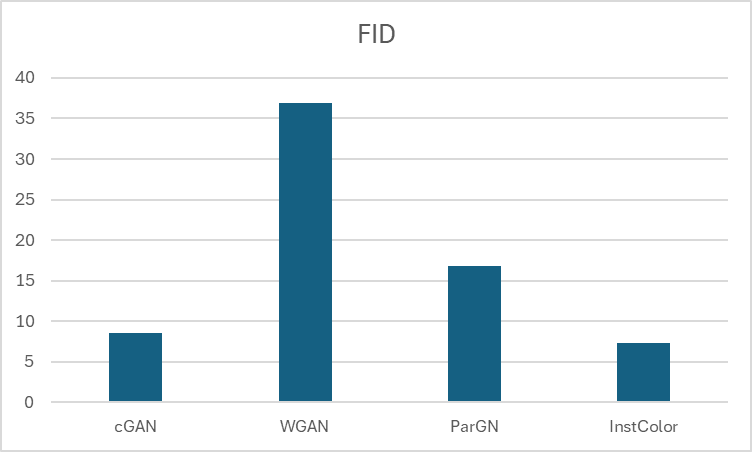
\includegraphics[width=0.75\linewidth]{imgs/fid_corrected.png}
    \caption{Stupčasti dijagram FID-ova modela}
    \label{fig:fid_comp}
\end{figure}


Kao što možemo vidjeti na prikazanom stupčastom dijagramu \ref{fig:fid_comp}, naš model (cGAN) ima značajno bolji iznos mjere FID od modela WGAN\cite{pix2pixwgan} i ParGN\cite{kumar2022paracolorizer}, ali ne toliko dobar kao model InstColor\cite{Su_2020_CVPR}. To bi mogao biti rezultat ekstrakcije značajki objekata iz slika koje provodi model InstColor\cite{Su_2020_CVPR}.

\begin{figure}[H]
    \centering
    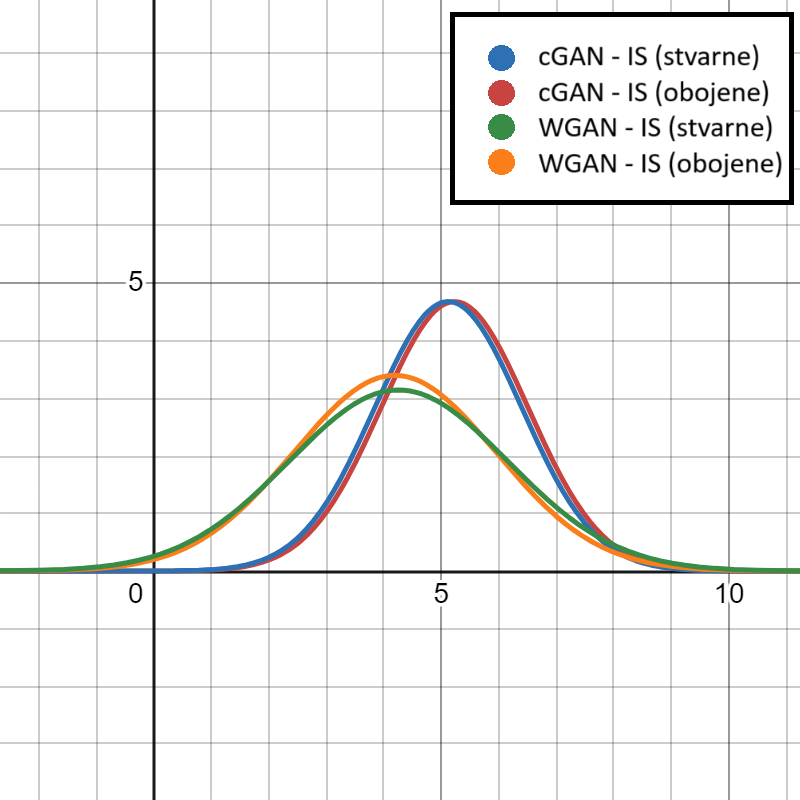
\includegraphics[width=0.75\linewidth]{imgs/is_comp.png}
    \caption{Graf IS-ova modela}
    \label{fig:is_comp}
\end{figure}

Kao što možemo vidjeti na grafu \ref{fig:is_comp}, naš model (cGAN) ima veći iznos mjere IS od modela WGAN\cite{pix2pixwgan}, uz manju standardnu devijaciju. Prema tome, naše obojene slike sličnije su stvarnim slikama u usporedbi s obojenim slikama dobivenim modelom WGAN\cite{pix2pixwgan}. Model WGAN\cite{pix2pixwgan} ima manju razliku središnje vrijednosti između stvarnih i obojenih slika iznosa $0.0915$, dok model cGAN ima razliku iznosa $0.1096$. Ipak, može se reći da cGAN ima bolji iznos mjere IS zbog znatno manje standardne devijacije, kao i općenito većeg iznosa.

\section{Zaključak}
% 7. Zaključak

Razvijen je relativno jednostavan model, koji se može naučiti na osobnim računalima s grafičkim karticama. Bojenje je donekle uspješno, kao što se moglo vidjeti na slikama \ref{fig:slike_skup} i \ref{fig:slike_vlastite}. Naučeni model vrlo dobro boji nijanse zelene i smeđe, kao i ljudsku kožu, ali ima problema sa šarenim površinama. Ova svojstva vezana su uz korišteni skup podataka za učenje.

Koristeći mjere dobrote FID i IS, vidljivo je da je model usporediv, ako ne i bolji, od sličnih modela za bojenje crno-bijelih slika. Prema mjeri dobrote FID, model je bolji od modela WGAN\cite{pix2pixwgan} i ParGN\cite{kumar2022paracolorizer}, a malo lošiji od modela InstColor\cite{Su_2020_CVPR} koji izlučuje značajke slika prije bojenja. Prema mjeri dobrote IS, model je bolji od modela WGAN\cite{pix2pixwgan}.

Za daljnja istraživanja, može se koristiti više procesorske snage grafičkog procesora (GPU snage) kako bi se model učio veći broj epoha. Povećanje skupa podataka također bi poboljšalo model - na primjer, model bi se mogao učiti na skupu podataka ImageNet\cite{deng2009imagenet}. Dodatno, mogu se isprobati modifikacije arhitekture, kao korištenje WGAN-a umjesto cGAN-a. Uz ovo, mogu se isprobati i potpuno drugačije arhitekture poput difuzijskih modela\cite{sohl2015deep}.

	\bibliography{literatura}
	\bibliographystyle{ieeetr}
        \nocite{*}
\end{document}
